

\section{Overview and Key Ideas}
\label{sec:overview}


In this section, we provide a brief outline of the basics of
Separation Logic (SL) and its inductive predicates. Next, we explain
how to use the existing ILP system \popper~\cite{cropper2021learning}
to synthesise such predicates from \emph{both positive and negative}
examples, and how we handle with learning from positive examples only.
%
We conclude with the high-level workflow of our SL predicate
synthesiser \tool.

\subsection{Inductive Predicates in Separation Logic}
\label{sec:sl}

\begin{figure}
  \centering
%  \belowcaptionskip=-10pt
%  \abovecaptionskip=5pt
  \includegraphics[width=0.8\textwidth]{figure/sll.pdf}
% \setlength{\abovecaptionskip}{0pt}

  \caption{Memory layout of a singly linked list.}
  \label{fig:sll}
\end{figure}
% 
Consider a schematic memory layout depicted in \autoref{fig:sll}
corresponding to a singly linked list (SLL).
%
The list has a recurring structure with each of its elements
represented by a consecutive pair of memory locations (the ``head''
one referred to by a pointer variable~\code{x}), the first one storing
its data value (or \emph{payload})~\code{v} and the second containing
the address \code{y} of the tail of the list. 
%
Knowing these shape constraints, the entire list can be traversed
recursively by starting from the head and following the tail pointers.
% thus, getting access to its payload.


The idea of defining the repetitive shape of a heap-based linked
structure, such as SLL, is precisely captured by Separation Logic and
its inductive (\ie, well-founded recursive) predicates. One encoding
of an SLL heap shape via the SL predicate \code{sll} is given below:

% The idea of defining the repetitive shape of heap-based linked
% structures
% %, such as SLL,  %for page break reason
% is captured by Separation Logic and
% its inductive (\ie, well-founded recursive) predicates. One
% encoding
% of an SLL heap shape   is given via the SL predicate:

\begin{lstlisting}
  pred sll(loc x, set s) where
    | x = 0 $\Rightarrow$ { s = {}; emp }
    | x $\neq$ 0 $\Rightarrow$ { s = {v} $\cup$ s1; x $\mapsto$ v * (x+1) $\mapsto$ y * sll(y, s1) }
\end{lstlisting}

\noindent
%
The predicate \code{sll} is parameterised by a location (\ie, pointer variable)
\code{x} and a payload set of the data structure
\code{s};
%
% \is{We could use algebraic lists to encode payloads instead of sets.
%   We should either address it or explain our choice.}
%
it holds true for any
\emph{heap fragment} that follows the shape of a linked list (and
contains no extra heap space).
%
What exactly that shape is, is defined by the two \emph{clauses} (\aka
constructors) of the predicate. 
%
The first one handles the case when \code{x} is a null-pointer,
constraining the payload set \code{s} of the list to be empty
(\code{\{\}}); the same holds for the list-carrying heap---which is
denoted by a standard SL assertion \code{emp}.\footnote{For
  simplicity, our examples use mathematical sets to encode the data
  payload, assuming uniqueness of the elements, instead of, \eg, an
  algebraic list. This is not a conceptual or practical limitation of
  our approach, as we will show in \autoref{sec:done}.}
%
The second clause describes a more interesting case, in which \code{x}
is not null, and so the payload can be split to an element \code{v}
and the residual payload \code{s1} (for simplicity of this example, we
assume that all elements of the list are unique).
%
Furthermore, the heap carrying the list is specified to have two
consecutive locations, \code{x} and \code{x + 1}, storing \code{v}
and some (existentially quantified) pointer value \code{y}, as denoted
by the SL \emph{points-to} notation $\mapsto$.
%
Finally, the rest of the SLL-carrying heap is 
the recursive occurrence of the same predicate \code{sll(y, s1)} (with
different arguments), thus replicating the recursive structure of the
layout from \autoref{fig:sll}.
%
% The heap-related constraints appearing after the semicolon in the
% clauses are traditionally referred to as \emph{spatial},
% while the remaining constraints (such as, \eg, the statement \code{s
%   == \{\}} constraining the empty list payload) are usually called
% \emph{pure}.



The logical connective \code{*} appearing in the second clause of the
\code{sll} predicate is known as the \emph{separating conjunction}
(sometimes pronounced ``and separately'') and is the main enabling
feature of Separation Logic~\cite{OHearn-al:CSL01}.
%
It implicitly constrains the symbolic heaps it connects in a spatial
assertion to have \emph{disjoint} domains.
%
Specifically, in this example it implies that the heap fragment
captured by \code{sll(y, s1)} does not contain memory locations
referred to by either \code{x} or \code{x+1}.
%
Such disjointness constraint  is what makes it
possible to avoid extensive reasoning about aliasing when using SL
specifications, making them \emph{modular}, \ie, holding true in the
context of any heap that is larger than what is affected by the
specified program.
%


% \subsection{\popper an ASP-based ILP system}

% \pagebreak

% \vspace{-5pt}
  
\subsection{From  Memory Graphs to Heap Predicates}
% \subsection{Synthesising Heap Predicates via ILP} maybe?
\label{sec:popper}

Our goal is to synthesise inductive SL predicates from examples of
concrete memory graphs.
%
To do so, we phrase both SL predicates and the memory graphs that
satisfy them in terms of Logic Programming. For example, the \prolog
predicate below defines a sorted singly linked list:
%
\begin{minted}[fontsize=\small]{prolog}
  srtl(X, S) :- empty(S), nullptr(X).
  srtl(X, S) :- next(X,Y), value(X,V), srtl(Y,SY), min_set(V,S), insert(SY,V,S).
\end{minted}
%
The predicate above defines a sorted singly linked list by enhancing
the ordinary singly linked list predicate with the constraint
\pcode{min_set(V, S)} that states that the value \pcode{V} is equal to
the smallest value in the set \pcode{S}. The \pcode{insert(S1, V, S)}
and \pcode{empty(S)} (\ie, \pcode{s == {v} ++ s1} and \pcode{s == {}}
in the SLL example) are defined using \prolog built-in predicates that
correspond to ordinary functions in set theory.
%
Other \prolog-style predicates used in the synthesised SL solutions
are data-structure specific and are extracted from the user-provided
memory graphs.
%
We leave till later (\autoref{sec:sldomain}) the issue of ensuring
that a \prolog predicate is also a \emph{valid} SL predicate in the
sense that it does not use SL connectives in a contradictory way,
allowing one to derive falsehood from its definition.


%
% Most of the predicates contributing to the definition of \code{srtl}
% come from predefined vocabularies, which the synthesiser will be aware
% of. During the search, it will be looking for definitions that can fix
% a number of clauses and combine available constraints, using the
% user-provided examples to validate its guesses.
%

\begin{figure}[t]
%\vspace{-15pt}
\centering
% \scalebox{0.75}{{\small{
\begin{tabular}{c}
    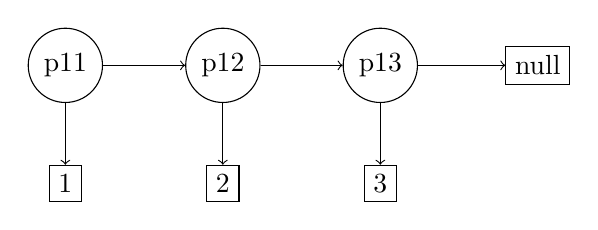
\begin{tikzpicture}
        \node[circle, draw] (n1) at (0,1.5) {p11};
        \node[circle, draw] (n2) at (2,1.5) {p12};
        \node[circle, draw] (n3) at (4,1.5) {p13};
        \node[draw] (null) at (6,1.5) {null};
        \node[draw] (v1) at (0,0) {1};
        \node[draw] (v2) at (2,0) {2};
        \node[draw] (v3) at (4,0) {3};
        \draw[->] (n1) --  node [above,midway] {\mynext} (n2);
        \draw[->] (n2) --  node [above,midway] {\mynext} (n3);
        \draw[->] (n3) --  node [above,midway] {\mynext} (null);
        \draw[->] (n1) --  node [midway] [above,midway,sloped] {\myvalue} (v1);
        \draw[->] (n2) --  node [midway] [above,midway,sloped] {\myvalue} (v2);
        \draw[->] (n3) --  node [midway] [above,midway,sloped] {\myvalue} (v3);
    \end{tikzpicture}
\\
\\
  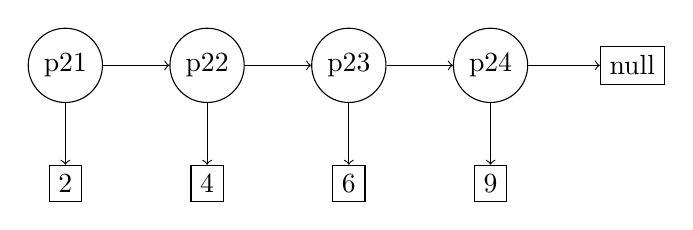
\begin{tikzpicture}
        \node[circle, draw] (n1) at (0,1.5) {p21};
        \node[circle, draw] (n2) at (1.8,1.5) {p22};
        \node[circle, draw] (n3) at (3.6,1.5) {p23};
        \node[circle, draw] (n4) at (5.4,1.5) {p24};
        \node[draw] (null) at (7.2,1.5) {null};
        \node[draw] (v1) at (0,0) {2};
        \node[draw] (v2) at (1.8,0) {4};
        \node[draw] (v3) at (3.6,0) {6};
        \node[draw] (v4) at (5.4,0) {9};
        \draw[->] (n1) --  node [above,midway] {\mynext} (n2);
        \draw[->] (n2) --  node [above,midway] {\mynext} (n3);
        \draw[->] (n3) --  node [above,midway] {\mynext} (n4);
        \draw[->] (n4) --  node [above,midway] {\mynext} (null);
        \draw[->] (n1) --  node [above,midway,sloped] {\myvalue} (v1);
        \draw[->] (n2) --  node [above,midway,sloped] {\myvalue} (v2);
        \draw[->] (n3) --  node [above,midway,sloped] {\myvalue} (v3);
        \draw[->] (n4) --  node [above,midway,sloped] {\myvalue} (v4);
    \end{tikzpicture}
\end{tabular}
}}
}
{\small{
\begin{tabular}{c}
    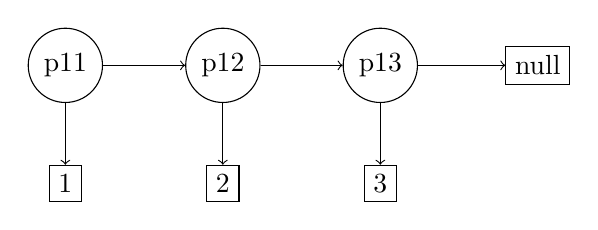
\begin{tikzpicture}
        \node[circle, draw] (n1) at (0,1.5) {p11};
        \node[circle, draw] (n2) at (2,1.5) {p12};
        \node[circle, draw] (n3) at (4,1.5) {p13};
        \node[draw] (null) at (6,1.5) {null};
        \node[draw] (v1) at (0,0) {1};
        \node[draw] (v2) at (2,0) {2};
        \node[draw] (v3) at (4,0) {3};
        \draw[->] (n1) --  node [above,midway] {\mynext} (n2);
        \draw[->] (n2) --  node [above,midway] {\mynext} (n3);
        \draw[->] (n3) --  node [above,midway] {\mynext} (null);
        \draw[->] (n1) --  node [midway] [above,midway,sloped] {\myvalue} (v1);
        \draw[->] (n2) --  node [midway] [above,midway,sloped] {\myvalue} (v2);
        \draw[->] (n3) --  node [midway] [above,midway,sloped] {\myvalue} (v3);
    \end{tikzpicture}
\\
\\
  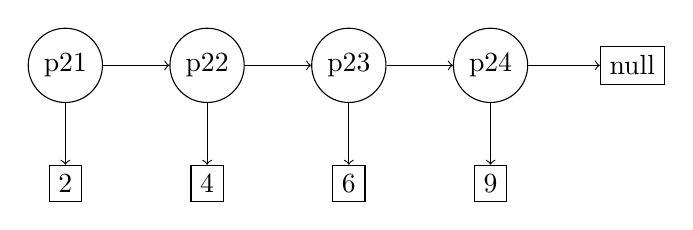
\begin{tikzpicture}
        \node[circle, draw] (n1) at (0,1.5) {p21};
        \node[circle, draw] (n2) at (1.8,1.5) {p22};
        \node[circle, draw] (n3) at (3.6,1.5) {p23};
        \node[circle, draw] (n4) at (5.4,1.5) {p24};
        \node[draw] (null) at (7.2,1.5) {null};
        \node[draw] (v1) at (0,0) {2};
        \node[draw] (v2) at (1.8,0) {4};
        \node[draw] (v3) at (3.6,0) {6};
        \node[draw] (v4) at (5.4,0) {9};
        \draw[->] (n1) --  node [above,midway] {\mynext} (n2);
        \draw[->] (n2) --  node [above,midway] {\mynext} (n3);
        \draw[->] (n3) --  node [above,midway] {\mynext} (n4);
        \draw[->] (n4) --  node [above,midway] {\mynext} (null);
        \draw[->] (n1) --  node [above,midway,sloped] {\myvalue} (v1);
        \draw[->] (n2) --  node [above,midway,sloped] {\myvalue} (v2);
        \draw[->] (n3) --  node [above,midway,sloped] {\myvalue} (v3);
        \draw[->] (n4) --  node [above,midway,sloped] {\myvalue} (v4);
    \end{tikzpicture}
\end{tabular}
}}

\\[5pt]
\begin{minted}[fontsize=\small]{prolog}
  pos(srtl(p11,[1,2,3])). pos(srtl(p21,[2,4,6,9])).

  % Encoding of the first memory graph from Fig.2
  next(p11, p12). next(p12, p13). next(p13, null). 
  value(p11, 1).  value(p12, 2).  value(p13, 3).

  % Encoding of the second memory graph from Fig.2
  next(p21, p22). next(p22, p23). next(p23, p24). next(p24, null).
  value(p21, 2).  value(p22, 4).  value(p23, 6).  value(p24, 9).
\end{minted}

%\setlength{\abovecaptionskip}{5pt}
% \setlength{\belowcaptionskip}{-10pt}
    \caption{Positive examples of sorted list heap graphs, with the corresponding logic encoding.}
    \label{fig:sorted-list}
\end{figure}

The top of \autoref{fig:sorted-list} shows two memory graphs of sorted
lists that can be used to synthesise \pcode{srtl()}.
%
For a more natural representation in terms of Logic Programming, we
use Java-style naming of structure components, \ie, fields such as
{\small{\textsf{value}}} and {\small{\textsf{next}}} instead of
C-style integer pointer offsets;
%
these fields provide the data-specific predicates (\ie, \pcode{next()}
and \pcode{value()}) to the synthesiser. In the bottom of
\autoref{fig:sorted-list}, we provide the corresponding logic
representations of the inputs to the synthesiser, consisting of
positive examples (\ie, instances of the sought predicate that are
expected to be true), and the background knowledge (\ie, encoding of
the corresponding memory graphs) that should be used to derive those
examples using predicate candidates.
%
Given all this information, a synthesiser should be able to generate
the predicate \pcode{srtl()} that satisfies the positive examples.
%
That is, using the traditional program synthesis from
input-output pairs as an analogy~\cite{GulwaniPS17}, the facts in
background knowledge (\eg, \pcode{next(p11, p12)}) are inputs, the
examples (\eg, \pcode{pos(srtl(p11, [1,2,3]))}) are the outputs, and
the solution is the program (\ie, the predicate) to be synthesised.

% \begin{figure}[t]
% % \setlength{\belowcaptionskip}{-10pt}
% % \setlength{\abovecaptionskip}{5pt}
% \begin{minted}[fontsize=\small]{prolog}
%   pos(srtl(p11,[1,2,3])). pos(srtl(p21,[2,4,6,9])).

%   % Encoding of the first memory graph from Fig.2
%   next(p11, p12). next(p12, p13). next(p13, null). 
%   value(p11, 1).  value(p12, 2).  value(p13, 3).

%   % Encoding of the second memory graph from Fig.2
%   next(p21, p22). next(p22, p23). next(p23, p24). next(p24, null).
%   value(p21, 2).  value(p22, 4).  value(p23, 6).  value(p24, 9).
% \end{minted}
% \caption{Positive examples for \code{srtl} in \popper. \todo{merge to one figure?}}
% \label{fig:examples}
% \end{figure}


\subsection{Predicate Synthesis via Answer Set Programming}
\label{sec:asp}

We observe that the synthesis of SL predicates can be regarded as a
Logic Programming synthesis task, studied extensively in the field of
Inductive Logic Programming
(ILP)~\cite{Muggleton91,cropper2020turning}. 
%
In ILP, the synthesis of definition is done by generating hypotheses
(\ie, predicates) and testing them against the provided examples.
%
Efficient generation of hypotheses in ILP is typically implemented
using Answer Set Programming (ASP)~\cite{gebser2022answer,aspguide}, a
constraint solving-based search-and-optimisation methodology that
allows for effectively pruning the search space of candidate
definitions and is used in many state-of-the-art ILP systems:
\aspal~\cite{corapi2011inductive}, \popper\cite{cropper2021learning},
and \aspsyn~\cite{bembenek2023smt}.

To see how ASP can be used for synthesising logic predicates, we first
provide a brief introduction to its principles using very basic
examples. 
%
Considered a declarative logic programming paradigm, ASP can be
regarded as a syntactic extension of \tname{Datalog}, but with a
different semantics called \emph{stable model
  semantics}~\cite{gelfond1988stable}. The output of an ASP program is
a set of \emph{models} (\ie, so-called answer set) that satisfy the
program constraints. A (normal) ASP program consists of a set of
\emph{clauses} that are composed of a head (on the left of
$\leftarrow$) and a body (on the right of $\leftarrow$) as:
%
\[
   a\ \leftarrow\ b_1,\ldots\ b_m,\ \neg\ c_1,\ \ldots,\ \neg\ c_n.
\]
%
which can be read as "if $b_1,\ldots\ b_m$ are true and
$c_1,\ \ldots,\ c_n$ are false, then $a$ is true". 
The statements $a,~b_i,~c_i$ are called \emph{literals} and are
declared in the format of \pcode{pred_name(X1, ..., Xn)} (\ie, a
predicate with arity $n$). 
%
A clause is called an \emph{integrity constraint} when its head (\ie,
the statement on the left-hand side of $\leftarrow$) is empty, which
means it is inconsistent if the body is true; a clause is called a
\emph{fact} when its body is empty, which means the head is always
true.

Instead of describing the formal definition of a stable
model, we show simple examples of ASP program and the corresponding
answer sets below:
%
\[
  % \begin{footnotesize}
    \begin{tabular}{c|l|l}
      No. &ASP Program&Answer Sets\\\hline
      1&\pcode{a :- b. b.}&\pcode{{a,b}}\\
      2&\pcode{a :- not b. b.}&\pcode{{b}}\\
      3&\pcode{a :- not b. b :- not a.}&\pcode{{a},{b}}\\
      4&\pcode{a :- not b. b :- not a. :- a.}&\pcode{{b}}\\
    \end{tabular}
  % \end{footnotesize}
\]
%
The arity of the literals \pcode{a} and \pcode{b} is 0, and
\pcode{:-}, \pcode{not} in the programs mean $\leftarrow$ and $\neg$
correspondingly.
%
The programs in the table above and their answer sets should be
interpreted as follows.

\begin{itemize}
\item Program 1 is a simple program with a rule (general clause)
  \pcode{a :- b} and the fact \pcode{b} postulating that \pcode{b} is
  true. The answer set is \pcode{{a,b}} meaning that \pcode{a} and
  \pcode{b} can be true together, given the constraints.
%
\item Program 2 is similar to Program 1, but with the rule \pcode{a :-
    not b} instead, which means \pcode{a} is true when \pcode{b} is
  false. The answer set is \pcode{{b}}, no clause is making \pcode{a}
  true.
%
\item Program 3 is a program with two rules. The answer set is
  \pcode{{a},{b}} because \pcode{a} is true when \pcode{b} is false,
  and \pcode{b} is true when \pcode{a} is false, so the answer set is
  the combination of the two cases.
%
\item Program 4 is extended from Program 3 with another clause, that
  is an integrity constraint \pcode{:- a} forcing \pcode{a} to be false. The answer set is \pcode{{b}}
  because \pcode{b} is true when \pcode{a} is false, and the program is
  consistent only in this case (in contrast with Program~3).
\end{itemize}

\noindent
%
As Program 4 demonstrates, the integrity constraint can be used to
prune the answer sets---a very useful feature for synthesis tasks
(more discussion on ASP versus SMT is in \autoref{sec:related}).

Each program above can be regarded as an \emph{enumeration in the
  powerset} of the set with two elements, \pcode{a} and \pcode{b},
returning \emph{all sets} that satisfy the relations (\ie, the ASP
clauses) between the elements.
%
An ILP system, such as \popper~\cite{cropper2021learning}, relies on
an ASP solver to encode the enumerative search among all possible
combinations of literals to synthesise logic predicates.

As a concrete example of ILP via ASP, consider synthesising the
definition of a predicate \pcode{plus_two(A, B)} using six literals:
\pcode{succ(A, A)}, \pcode{succ(A, C)}, \pcode{succ(B, A)},
\pcode{succ(B, B)}, \pcode{succ(B, C)}, and \pcode{succ(C, B)} to
build the body of the predicate, with examples \pcode{plus_two(1,3)}
and \pcode{plus_two(2,4)}.
%
An ASP-based synthesiser would try to find a definition of
\pcode{plus_two(A, B)} as a suitable subset of all their $2^6=64$
possible combinations.
%
While doing so, it would also make use of the natural restrictions
that can be encoded as integrity constraints, such as
%
(1)~no free variable is allowed in the body (hence \pcode{{succ(A, B), succ(C, B)}} is
not a valid answer set because \pcode{C} is free), and 
%
(2)~all input variables \pcode{A} and \pcode{B} should appear in the
body (hence \pcode{{succ(B, C)}} is not a valid synthesis candidate).
%
As we will show, such constraints are also useful for encoding the
domain-specific knowledge about validity of SL predicates, and can be
efficiently solved by ASP solvers.
%
% Finally, 
% answer set \pcode{{succ(A,C), succ(C,B)}} pass
% the input examples' test such as \pcode{plus_two(1,3)} and
% \pcode{plus_two(2,4)}.

Moreover, the incrementality of ASP solvers make it possible to
constrain the search space continuously~\cite{gebser2019multi}. For
instance, assume the following hypothesis is obtained during the
search:
%
\begin{minted}[fontsize=\small]{prolog}
  plus_two(A, B) :- succ(A, A), succ(B, B).
\end{minted}
%
% which corresponds to the answer set
% %
% \begin{minted}[fontsize=\scriptsize]{prolog}
%   head(0,srtl,(X,S)). body(0,value,(X,V)). body(0,min_set,(V,S)).
% \end{minted}
% %
% That is, the clause 0 has one head predicate \pcode{srtl(X, S)} and
% two body predicates \pcode{value(X, V)} and \pcode{min_set(V, S)}.

% MARK: should be 5 pages above
%
%
After testing it by \prolog against the examples, \popper finds that
none of the provided positive examples can be derived using this
solution.
%
As the result, other hypotheses that are more \emph{specialised} (\ie,
more constrained in the bodies) than it, such as the definition of
\pcode{plus_two()} below.
%
\begin{minted}[fontsize=\small]{prolog}
  plus_two(A, B) :- succ(A, A), succ(B, A), succ(B, B).
\end{minted}
%
will also entail no positive examples.
%
To this end, with the help of ASP, a classic ILP performs search for
a candidate hypothesis that passed all tests and has the smallest size
(\ie, number of literals in the predicate). Such \emph{optimal}
hypothesis for our example is the synthesised solution:
%
\begin{minted}[fontsize=\small]{prolog}
  plus_two(A, B) :- succ(A, C), succ(C, B).
\end{minted}


\subsection{Synthesis without Negative Examples}
\label{sec:approach}

The classic ILP comes with an important limitation: in general, it
requires both \emph{positive} and \emph{negative} examples to learn a
predicate. As we explain below, the need for the latter kind of
examples makes it challenging to employ ILP \emph{as-is} as a
pragmatic approach for synthesising SL predicates.


\paragraph{Why Negative Examples are Necessary in ILP}

Let us get back to our examples with synthesising a sorted singly
linked list predicate from positive examples of memory graphs in
\autoref{fig:sorted-list}. 
%
With the conventional ILP, the learned hypothesis by \popper is as
follows, and it is not what we need:
%
\begin{minted}[fontsize=\small]{prolog}
  srtl(X, S) :- empty(S), nullptr(X).
  srtl(X, S) :- next(X, Y), value(X, V), insert(SY, V, S), srtl(Y, SY).
\end{minted}
%
The learned hypothesis does not define a sorted list,
but an ordinary (unsorted) singly linked list.
%
The reason is: in the absence of the negative example, this is a
consistent hypothesis that is smaller in size than the correct
definition of \code{srtl}.
So if we want to learn the correct predicate, we need to provide negative examples that are inconsistent with the incorrect hypothesis, such as
%
\begin{minted}[fontsize=\small]{prolog}
  neg(srtl(p11, [1,2,3])).
  % Encoding of a negative example
  next(n1, n2). next(n2, n3). next(n3, null). 
  value(n1, 2). value(n2, 1). value(n3, 3).
\end{minted}
%
which is a singly linked but not sorted list. To summarise, when
performing synthesis via classic ILP, negative examples are necessary
to avoid the predicate being \emph{too general}.
%



\paragraph{Challenges in Obtaining Negative Examples.}
What makes things worse is that ILP systems rely on
\emph{representative} negative examples to correctly prune the
generality, which are hard to obtain automatically.
%
% The difference between positive and negative examples is that, a
% good set of positive examples only needs to guarantee that all
% instances follow the predicate, while a good set of negative
% examples needs to cover all possible ways that the predicate can be
% wrong (\ie, being too general).
%
The difference between positive and negative examples is that, a good
set of positive examples (\(\mathbf{Pos}\)) only needs to guarantee
that all instances follow the predicate (\(\mathcal{P}\)), while a
good set of negative examples (\(\mathbf{Neg}\)) need to be much more
elaborated, so it could cover any possible way in which the predicate
can be wrong. This difference is expressed by the following
quantifications:
\[
  \forall \mathbf{e^+} \in \mathbf{Pos}, \mathcal{P}(\mathbf{e^+})
  \quad \text{vs.} \quad
  \forall \mathcal{P'} \subset \mathcal{P}, \exists \mathbf{e^-} \in \mathbf{Neg},  \mathcal{P'}(\mathbf{e^-}) \land \neg\mathcal{P}(\mathbf{e^-})
\]
That is, unlike a good positive example set, which is only quantified
over the examples, a good negative example set is quantified over the
\emph{predicates} and the examples, which makes it much harder to
achieve. As a concrete example of this phenomenon, imagine learning a
predicate for balanced binary trees.
%
A good set of negative examples would contain instances where
(a)~the height of the left subtree is too large, (b)~the height of the
right subtree is too large, (c)~the imbalance manifests recursively in
both left and right subtrees.
%
Without all these rather specific negative instances, it is possible
to learn a predicate with a constraint on the subtrees
\pcode{height(Left) <= height(Right) + 1}, which is not wrong but is
imprecise. This is not just an issue for SL predicates domain, but
also for general logical learning, witnesses by the fact that in
existing ILP benchmarks~\cite{cropper2021learning,thakkar2021example}
and specification mining framework \cite{10.1145/3622876} high-quality
negative examples are often crafted manually.

%\vspace{-3pt}
\begin{figure}[t]
%  \abovecaptionskip=4pt
%  \belowcaptionskip=-10pt
  \centering
  \includegraphics[width=0.5\textwidth]{figure/examples.pdf}
  \caption{The effect of positive and negative examples on search.}
      \label{fig:illustration}
\end{figure}


This state of affairs brings us to the two key novel ideas of this
work that enable efficient synthesis of SL predicates only from
positive examples.

\subsubsection{Key Idea 1: Learning with Specificity.}
\label{sec:most-specific}


%
As discussed above, without negative examples a solution delivered by
\popper, while valid, may not be specific enough.
%
To provide more intuition on the space of possible design choices in
finding the best solution, together with the reason why positive-only
learning is possible, let us consider the illustration in
\autoref{fig:illustration}. The ``up''/``down'' in this figure
(informally) means ``more general/specific'', where the top/bottom
are constant True/False (\ie, the lattice is defined by
subsumption~\cite{muggleton1995inverse}).
%
Providing two positive examples, \code{p1} and \code{p2}, restricts
the search space for the solution hypothesis to the intersection of
their own spaces, with the most general one chosen as the solution.
%
Adding a negative example \code{n1} provides more restrictions, thus
allowing for more specific most-general solution.
%
From this diagram, one can see that, even without a negative example,
we can have a
\emph{tighter}~\cite{DBLP:journals/pacmpl/AstorgaSDWMX21} solution
(\ie, with stronger restrictions given the same number of clauses) if
we consider not the most general, but the most specific candidate in
the intersection of the search spaces defined by \code{p1} and
\code{p2} (generally, positive examples only).

Therefore, the basic idea of our positive-only learning is: to learn
\emph{the most specific} predicate admitting all provided examples.
The only problem is: what is the definition of ``specificity''? As the
opposite of ``generality'' (the program with the smallest number of
constraints), it is not practical to take the \emph{largest}
hypothesis as the most specific, as it would lead to \emph{redundant}
constraints.
%
As an example, consider the following valid formulation of the sorted
linked list predicate that requires, in its second clause, that
\code{T} = \code{SY}~$\cup \set{\codeinmath{V}}$ and \code{S} =
\code{T}~$\cup \set{\codeinmath{V}}$:
%
\begin{minted}[fontsize=\small]{prolog}
srtl(X, S) :- empty(S), nullptr(X).
srtl(X, S) :- next(X, Y), value(X, V), srtl(Y, SY), insert(SY, V, T), insert(T, V, S).
\end{minted}
%
Clearly, the last conjunction \pcode{insert(T, V, S)} is redundant and
can be removed because of the properties of the \pcode{insert(...)}
predicate.
%


To eliminate such candidates with redundancies, our approach for
positive-only learning encodes intrinsic logical properties of customised
predicates to \emph{minimise} the generated SL predicates.
%
Our tool comes with a pre-defined collection of properties of
predicates for common arithmetic (\eg, calculation, comparison) and
set operations (\eg, insertion, union) that are included into the
synthesis automatically.
%
More customised predicates can be added
by the user (with additional clause minimisation rules). 
%
After performing the minimisation hinted above (detailed in
\autoref{sec:normalise}), we define the \emph{specificity} of a predicate
candidate based on its size \wrt other available candidates
(\cf~\autoref{sec:tool}). The solution that is locally-optimal (\ie, the
strongest in the search space) will be adopted as the most specific predicate that is implied by
all the positive examples.



\subsubsection{Key Idea 2: Separation Logic-Based Pruning.}
\label{sec:pruning}



The domain of our synthesis, \ie, Separation Logic, provides effective
ways to prune the search space and accelerate the synthesis process. 
%
Postponing the detailed explanation of the optimisations until
\autoref{sec:SLsynthesis}, as an example, consider an important
property the separating conjunction stating that the fact
\code{x}~$\mapsto$~\code{a * y} $\mapsto$ \code{b} implies
\code{x}~$\neq$~\code{y} because of the disjointness assumption
enforced by \code{*}.
%
This property can be encoded as a pruning strategy via ASP integrity
constraints (\autoref{sec:asp}) that are generated by our tool for
each synthesis task.
%
% \begin{minted}[fontsize=\scriptsize]{prolog}
%  :- clause(C), pointer(X), #count{V: body_lit(C, next, (X, V))} > 1.
% \end{minted}
%
Even for a \emph{doubly linked list}, one of the simplest predicates
in our benchmark (\cf~\autoref{sec:done}), without such optimisations,
the synthesis time is increased from 3 to 339 seconds; the synthesis
of more complex predicates does not terminate in 20 minutes without
SL-specific pruning.

\subsection{Automatically Generating Positive Examples}

So far, we assumed that the positive examples are provided by the
user, in the format of memory graphs. 
%
In practice, one may expect that such examples can be obtained in a
more automated way, \eg, from the available programs that manipulate
with the respective data structures.
%
For instance, an existing work on shape analysis~\cite{le2019sling} uses
a debugger for extracting memory graphs from a program's execution,
with the assumption that (1)~the user indicates the line of code to
extract the memory graph, and (2)~an input for the program is provided.
%
Unfortunately, this rules out a large set of programs that
\emph{expect} a data structure rather than generate one: without a
suitable input we simply cannot run them to obtain a graph, and constructing
such input is a task not much easier than encoding a memory graph manually.

% However, considering a function "removing a certain element from a
% binary search tree", we cannot obtain the trees without a constructor
% function, thus the memory graphs cannot be extracted because of
% non-executability of the function itself.

To address this issue, we implemented \ggen---a tool that can
automatically generates positive example in the form of arbitrary valid
memory graphs of a data structure from the program that manipulates
with the structure, without requiring the user to provide any input.
%
The only assumption we make is that the program in question is
instrumented with test assertions, which can be used to filter out the
invalid memory graphs from the randomly generated ones. We further
show in \autoref{sec:verification} that \ggen can effectively generate
input graphs for synthesising SL predicates from real
heap-manipulating programs, reducing the specification burden for
proving their correctness.

% \vspace{-5pt}


\begin{figure}[!t]
  \centering
  % \abovecaptionskip=5pt
  % \belowcaptionskip=-15pt
      
      \begin{adjustbox}{width=0.96\textwidth}
        \section{Problem definition}
\label{sec:problem-def}

The first step in building and using a \CSE{} or SciML model is defining the problem scope: the model's intended purpose, application domain and operating environment, required quantities of interest (QoI) and their scales, and how prior knowledge informs model conceptualization.

\subsection{Model purpose}

\begin{essrec}[Specify prior knowledge and model purpose]
Define the model's intended use and document the essential model properties that must be satisfied. Document any known limitations and constraints of the chosen approach. This ensures appropriate data selection and physics-informed objectives while preventing model misuse outside its intended scope.
\end{essrec}

A SciML model's purpose, as discussed in Section~\ref{sec:scope}, dictates all subsequent modeling choices.
This purpose determines required outer-loop processes and essential properties.

To highlight the importance of specifying the target outer-loop process, consider a model used for explanatory modeling. An explanatory model must simulate all system processes, like ice-sheet thickness and velocity evolution. In contrast, a risk assessment model needs only decision-relevant quantities, like ice-sheet mass loss under varying emissions scenarios. Design and control models, meanwhile, have different requirements than those for risk assessment.
The model purpose dictates the data types and formulations needed to train a SciML model. The impact of this purpose on data requirements and physics-informed objectives varies by application domain. Thus, the exact model formulation should be chosen in light of these problem-specific considerations.


\subsection{Verification, calibration, validation and application domain}

\begin{essrec}[Specify verification, calibration, validation, and application domains]
Define the specific conditions under which the model will operate across the verification, calibration, validation, and prediction phases. These domains are specified by relevant boundary conditions, forcing functions, geometry, and timescales. Account for potential differences between these domains and address any data distribution shifts that could affect model performance. This ensures the selected model architecture and training data align with the intended use while preventing unreliable predictions when operating outside validated conditions.
\end{essrec}

The trustworthy development and deployment of a model (see Figure~\ref{fig:model-development}) requires using the model in regards to verification, calibration, validation, and application domains. These domains are defined by the conditions under which the model operates during these respective phases and must be defined before model construction because they determine viable model classes. Key features include boundary conditions, forcing functions, geometry, and timescales. For ice sheets, examples include surface mass balance, land mass topography, and ocean temperatures.

Each domain will often require the prediction of different quantities of interest under different conditions. Moreover the complexity of the processes being modeled typically increase when transitioning from verification to calibration, to validation to prediction. Additionally the amount of data to complement or inform the model decreases as we move through these domains. For example, the verification domain for our ice-sheet examplar predicts the entire state of the ice-sheet for simple manufactured or analytical solutions. The calibration domain predicts Humboldt Glacier surface velocity under steady-state preindustrial conditions. The validation domain predicts grounding-line change rates from the first decade of this century. The application domain predicts glacier mass change in 2100. Figure~\ref{fig:computational-domains} illustrates these distinct domains. When transitioning between domains, data shifts across domains must be considered. For example, a model trained only on calibration data from recent ice-sheet forcings may fail to predict ice-sheet properties under different future conditions.

\begin{figure}[htb]
    \centering
    \includegraphics[width=0.65\linewidth]{application-domain.pdf}
    \caption{Verification, validation, calibration and application domains.}
    \label{fig:computational-domains}
\end{figure}


\subsection{Quantities of interest}

\begin{essrec}[Carefully select and specify the quantities of interest]
Select and specify the model outputs (quantities of interest, QoI) required for the intended use, considering their form and scale. For risk assessment and design applications, identify the minimal set of QoIs needed for decision-making or optimization. For explanatory modeling, specify the broader range of QoIs needed to capture system behavior. This choice fundamentally determines the required model complexity, training data requirements, and computational approach needed to achieve reliable predictions.
\end{essrec}

Quantities of interest (QoI) are the model outputs required by users. Their form and scale depend on modeling purpose and application domain. We now discuss key considerations for QoI selection.

Risk assessment requires reproducing only decision-critical QoI. For ice-sheets, these include sea-level rise from mass loss and infrastructure damage costs. Design applications similarly need few QoI to evaluate objectives and constraints, like thermal and structural stresses in aerospace vehicles. Design models need accurate QoI predictions only along optimizer trajectories\footnote{For each design iteration the model may still need to be accurate across all uncertain model inputs}, while risk assessment models must predict across many conditions. Explanatory modeling demands more extensive QoI sets, such as complete ice-sheet depth and velocity fields for studying calving. Therefore, simple surrogates often suffice for risk assessment and design, but explanatory modeling may require operators or reduced order models.


\subsection{Model conceptualization}


\begin{essrec}[Select and document model structure]
Select a model structure that fits the model's purpose, domain, and quantities of interest based on relevant prior knowledge such as conservation laws or system properties. Document the alternative model structures considered and the reasoning behind the final selection, including how available resources and computational constraints influenced the choice. This systematic approach ensures the model balances usability, reliability, and feasibility while maintaining transparency about structural assumptions and limitations.
\end{essrec}

Model conceptualization, which follows problem definition, involves selecting model structure based on prior knowledge. While essential to \CSE{} model development~\cite{Jakeman_LN_EMS_2006}, this step requires clear identification of the application domain and relevant QoI.

Model structure selection draws on key prior knowledge: conservation laws, system invariances like rotational and translational symmetries. These guide method selection---for example, symplectic time integrators~\cite{ruth1983canonical} preserve system dynamics properties. Moreover, this knowledge informs and justifies the selection of candidate model structures.
A \CSE{} modeler chooses between model types like lumped versus distributed PDE models, and linear versus nonlinear PDEs. The optimal choice depends on application domain, QoI, and available resources. For example, linear PDEs may introduce more error but their lower computational cost enables better error and uncertainty characterization for tasks like optimal design.
Similar considerations guide SciML model selection. For example, Gaussian processes excel at predicting scalar QoI with few inputs and limited data, but become intractable for larger datasets without variational inference approximations~\cite{Liu_CO_KBS_2018}. In contrast, deep neural networks handle high-dimensional data but require large datasets. The intended use also shapes model structure and training, e.g., optimization applications require controlling derivative errors~\cite{bouhlel2020scalable,o2024derivative} to ensure convergence~\cite{cao2024lazy,luo2023efficient}. These approximation errors must be understood and quantified where possible.

\CSE{} has a strong history of using prior knowledge to formulate governing equations for complex phenomena and deriving numerical methods that respect important physical properties. However, all models are approximate and the best model must balance usability, reliability, and feasibility~\cite{Hamilton_PSFJEMS_2022}. While SciML methods can be usable and feasible, more attention is needed to establish their trustworthiness. In the following two sections, we discuss how \CSE{} V\&V can improve the trustworthiness of SciML research.

\section{Verification}
\label{sec:verification}

Verification increases the trustworthiness of numerical models by demonstrating that the numerical method can adequately solve the equations of the desired mathematical model and the code correctly implements the algorithm. Verification consists of code verification and solution verification, which enhance credibility and trust in the model's predictions. Code and solution verification are well-established in \CSE{} to reduce algorithmic errors. However, verification for SciML models has received less attention due to the field's young age and unique challenges. Moreoever, because SciML models heavily rely on data, unlike \CSE{} models, existing \CSE{} verification notions need to be adapted for SciML.

\subsection{Code verification}
\label{sec:code-verification}

\begin{essrec}[Verify code implementation with test problems]
Evaluate the SciML model's accuracy on simple manufactured test problems using verification data that is independent from training data. Assess how the model error responds to variations in training data samples and optimization parameters while increasing both model complexity and training data size. This systematic testing approach reveals implementation issues, quantifies the impact of sampling and optimization choices, and establishes confidence in the model's numerical implementation.
\end{essrec}

Code verification ensures that a computer code correctly implements the intended mathematical model. For \CSE{} models, this involves confirming that numerical methods and algorithms are free from programming errors (``bugs"). PDE-based \CSE{} models commonly use the method of manufactured solutions (MMS) to verify code on arbitrarily complex solutions. MMS substitutes a user-provided solution into the governing equations, then differentiates it to obtain the exact forcing function and boundary conditions. These solutions check if the code produces the known theoretical convergence rate as the numerical discretization is refined. If the observed order of convergence is less than theoretical, causes such as software bugs, insufficient mesh refinement, or singularities and discontinuities affecting convergence must be identified.

Code verification for SciML models is important but challenging due to the large role of data and nonconvex numerical optimization. Three main challenges limit code verification for many SciML models.
First, while theoretical analysis of SciML models is increasing~\cite{schwab2019deep,schwab2023deep,opschoor2022exponential,leshno1993multilayer,lanthaler2023curse,kovachki2021universal,kovachki2023neural}, many models like neural networks do not generally admit known convergence rates outside specific map classes~\cite{schwab2019deep,schwab2023deep,opschoor2022exponential,herrmann2024neural}, despite their universal approximation properties~\cite{hornik1989multilayer,cybenko1989approximation,leshno1993multilayer}.
Second, generalizable procedures to refine models, such as consistently refining neural-network width and depth as data increases, do not exist.
Finally, regardless of data amount and model unknowns, modeling error often plateaus at a much higher level than machine precision due to nonconvex optimization issues like local minima and saddle points~\cite{Dauphin_PGCGB_NIPS_2014,Bottouleon_CN_SIAMR_2018}.

Developing theoretical and algorithmic advances to address the three main challenges limiting code verification can substantially improve the trustworthiness of SciML models. Convergence-based code verification is currently possible only for certain SciML models with theory that bounds approximation errors in terms of model complexity and training data amount, such as operator methods~\cite{Turnage_et_al_arxiv_2024}, polynomial chaos expansions~\cite{Cohen_M_SMAIJCM_2017,xiu2002wiener}, and Gaussian processes~\cite{Burt_RV_PMLR_2019}.

For SciML models without supporting theory, convergence tests should still be conducted and reported. Studies providing evidence of model convergence engender greater trustworthiness than those that do not, even when the empirically estimated convergence rate cannot be compared to theoretical rates. For example, observing Monte Carlo-type sampling rates in a regime of interest for a fixed overparametrized model can provide intuition into whether the model should be enhanced.

To account for the heavy reliance of SciML models on training data optimization, code verification should be adapted in two ways.
First, report errors in the ML model for a given complexity and data amount for different realizations of the training data to quantify the impact of sampling error, which is not present in \CSE{} models.
Second, because most SciML algorithms introduce optimization error, conduct verification studies that artificially generate data from a random realization of an ML model, then compare the recovered parameter values with the true parameter values or compare the predictions of the learned and true approximations, or at the very least compare the predictions of the two models. Additionally, quantify the sensitivity of the SciML model error to randomness in the optimization by varying the random seed and initial guess passed to the optimizer (see Section~\ref{sec:loss-and-opt}).
All verification tests must employ test data or \emph{verification data}, independent of the training data, to measure the accuracy of the SciML model.


\subsection{Solution verification}

\begin{essrec}[Verify solution accuracy with realistic benchmarks]
Test the model's performance on well-designed, realistic benchmark problems that reflect the intended application domain. Quantify how the model error varies with different training data samples and optimization parameters. When feasible, examine error patterns across different model complexities and data amounts; otherwise, focus on verifying the specific configuration intended for deployment. This ensures the model meets accuracy requirements under realistic conditions while accounting for uncertainties in training and optimization.
\end{essrec}

Code verification establishes a code's ability to reproduce known idealized solutions, while solution verification, performed after code verification, assesses the code's accuracy on more complex yet tractable problems defined by more realistic boundary conditions, forcing, and data. For example, code verification of ice sheets may use manufactured solutions, whereas solution verification may use more realistic MISMIP benchmarks~\cite{Cornford_et_al_TC_2020}. In solution verification, the numerical solution cannot be compared to a known exact solution, and the convergence rate to a known solution cannot be established. Instead, solution verification must use other procedures to estimate the error introduced by the numerical discretization.

Solution verification establishes whether the exact conditions of a model result in the expected theoretical convergence rate or if unexpected features like shocks or singularities prevent it. The most common approach for \CSE{} models compares the difference between consecutive solutions as the numerical discretization is refined and uses Richardson extrapolation to estimate errors. A posteriori error estimation techniques that require solving an adjoint equation can also be used.

While thorough solution verification of CSE models is challenging, these difficulties are further amplified for SciML models. Currently, solution verification of SciML models simply consists of evaluating a trained model's performance using test data separate from the training data. However, this is insufficient as solution verification requires quantifying the impact of increasing data and model complexity on model error. Yet, unfortunately, performing a posteriori error estimation for many SciML models using techniques like Richardson extrapolation is difficult due to the confounding of model expressivity, statistical sampling errors, and variability introduced by converging to local solutions or saddle points of nonconvex optimization, making it challenging to monotonically decrease the error of SciML models such as neural networks. 

Until convergence theory for SciML models improves and automated procedures are developed to change SciML model hyperparameters as data increases, solution verification of SciML models should repeat the sensitivity tests proposed for code verification (Section~\ref{sec:code-verification}) with two key differences:
First, verification experiments used to generate verification data must be specifically designed for solution verification, as not all verification data equally informs solution verification efforts, similar to observations made when creating validation datasets for \CSE{} models~\cite{Oberkampf_T_PAS_2002}. See Section~\ref{sec:data-sources} for more information on important properties of verification benchmarks.
Second, while ideally the convergence of SciML errors on realistic benchmarks should be investigated, it may be computationally impractical. Thus, solution verification should prioritize quantifying errors using the model complexity and data amount that will be used when deploying the SciML model to its application domain.

\section{Validation}
\label{sec:validation}

Verification establishes if a model can accurately produce the behavior of a system described by governing equations. In contrast, validation assesses whether a \CSE{} model's governing equations---or data for SciML models---and the model's implementation can reproduce the physical system's important properties, as determined by the model's purpose.

Validation requires three main steps: (1) solve an inverse problem to calibrate the model to observational data; (2) compare the model's output with observational data collected explicitly for validation; and (3) quantify the uncertainty in model predictions when interpolating or extrapolating from the validation domain to the application domain. We will expand on these steps below.
But first note that the issues affecting the verification of SciML models also affect calibration and validation. Consequently, we will not revisit them here but rather will highlight the unique challenges in validating SciML models.

\subsection{Calibration}

\begin{essrec}[Perform probabilistic calibration]
Calibrate the trained SciML model using observational data to optimize its predictive accuracy for the application domain. Implement Bayesian inference when possible to generate probabilistic parameter estimates and quantify model uncertainty. Choose calibration metrics that account for both model and experimental uncertainties, and select calibration data strategically to maximize information content within experimental constraints. This approach enables reliable uncertainty estimation and optimal use of available observational data.
\end{essrec}

Once a \CSE{} model has been verified, it must be calibrated to match experimental data that contains observational noise. This calibration requires solving an inverse problem~\cite{Stuart_AN_2010}, which can be either deterministic or statistical (e.g., Bayesian). The deterministic approach formulates the inverse problem as a (nonlinear) optimization problem that minimizes the mismatch between model and experimental data. This formulation requires regularization to ensure well-posedness, typically chosen using the L-curve~\cite{hansen1999curve} or the Morozov discrepancy principle~\cite{anzengruber2009morozov}. The Bayesian approach replaces the misfit with a likelihood function based on the noise model, while using a prior distribution for regularization. This prior distribution ensures well-posedness while encoding typical parameter ranges and correlation lengths. We recommend Bayesian methods for calibration because they provide insight into the uncertainty of the reconstructed model parameters. 

The calibration of SciML operator, reduced-order, and hybrid CSE-SciML models is distinct from SciML training and follows similar principles to \CSE{} model calibration. These models are first trained using simulation data for solution verification. Next, observational data (called \emph{calibration data}) determines the optimal model input values that match experimental outputs. For instance, calibrating a SciML ice-sheet model such as that of Ref.~\cite{He_PKS_JCP_2023} requires finding optimal friction field parameters of a trained SciML model, which best predict observed glacier surface velocities, given the noise in the observational data.

Calibration typically improves a model's predictive accuracy on its application domain, but the informative value of calibration data varies significantly. Therefore, researchers should select calibration data strategically to maximize information content within their experimental budget. See Section~\ref{sec:data-sources} for further discussion on collecting informative data.

\subsection{Model validation}

\begin{essrec}[Validate model against purpose-specific requirements]
Define validation metrics that align with the model's intended purpose. Then validate the model using independent data that was not used for training or calibration, ensuring it captures essential physics and boundary conditions of interest. If validation reveals inadequate performance, iterate by collecting additional training data, refining the model structure, or gathering more calibration data until the model achieves satisfactory accuracy for its intended application. This systematic approach will help ensure the model meets stakeholder requirements while maintaining scientific rigor.
\end{essrec}

Model validation is the ``substantiation that a model within its domain of applicability possesses a satisfactory range of accuracy consistent with the intended application of the model''~\cite{Refsgaard_H_AWR_2004}. Validation involves comparing computational results with observational data, then determining if the agreement meets the model's intended purpose~\cite{Lee_et_all_AIAA_2016}. For \CSE{} models with unacceptable validation agreement, modelers must either collect additional calibration data or refine the model structure until reaching acceptable accuracy. SciML models follow a similar iterative process but offer an additional option: to collect more training data.

Model validation must occur after calibration and requires independent data not used for calibration or training. For our conceptual ice-sheet model, calibration matches surface velocities assumed to represent pre-industrial conditions, while validation assesses the calibrated model's ability to predict grounding line change rates at the start of this decade. Performance metrics must target the specific modeling purpose. For optimization tasks, metrics should measure the distance from true optima obtained via the SciML model or bound the associated error~\cite{cao2024lazy}. For uncertainty estimation, metrics should quantify errors in uncertainty statistics through moment discrepancies or density-based measures like (shifted) reverse and forward Kullback--Leibler divergences.
For explanatory SciML modeling, validation metrics must also assess physical fidelity: adherence to physical laws, conservation properties (such as mass and energy), and other constraints. As with verification, the validation concept should encompass \emph{data validation}, particularly whether training data adequately represents the application space.

Validation determines whether a model is acceptable for its specific purpose rather than universally correct. The definition of acceptable is subjective, depending on validation metrics and accuracy requirements established by model stakeholders in alignment with the problem definition and model purpose (see Section~\ref{sec:problem-def}). Moreoever, validation itself does not constitute final model acceptance, which must be based on model accuracy in the application domain, as discussed in Section~\ref{sec:prediction}.

Two additional considerations complete our discussion of model validation. First, this validation differs from the concept of \emph{cross validation}, which estimates ML model accuracy on data representative of the training domain during development. The validation described here assesses accuracy in a separate validation domain. Second, validation data varies in informative value. Validation experiments should ``capture the essential physics of interest, including all relevant physical modeling data and initial and boundary conditions required by the code''~\cite{Oberkampf_T_NED_2008}. Most critically, validation data must remain independent from training and calibration data. 

\subsection{Prediction}
\label{sec:prediction}

\begin{essrec}[Quantify prediction uncertainties]
Assess and quantify all sources of uncertainty affecting model predictions in the application domain, including numerical approximation errors, input and parameter uncertainties, sampling errors from finite training data, and optimization errors. Propagate these uncertainties through the model using appropriate techniques to estimate relevant statistics that match validation criteria. Define acceptance thresholds for prediction uncertainty to ensure the model's reliability for its intended use while acknowledging inherent limitations in uncertainty quantification.
\end{essrec}

Although extensive data may be available for model calibration, validation data is typically scarcer and may not represent the model's intended application domain. According to Schwer~\cite{Schwer_EWC_2007}, ``The original reason for developing a model was to make predictions for applications of the model where no experimental data could, or would, be obtained.'' Therefore, minimizing validation metrics at nominal conditions cannot sufficiently validate a model. Modelers must also quantify accuracy and uncertainty when predictions are extrapolated to the application domain.

SciML models, like \CSE{} models, are subject to numerous sources of uncertainty. The impact of these uncertainties on model predictions must be quantified. Several sources of uncertainty affect \CSE{} models. These include: numerical errors, from approximating the solution to governing equations; input uncertainty arises, which is caused by inexact knowledge of model inputs; parameter uncertainty, which stems from inexact knowledge of model coefficients; and model structure error representing the difference between the model and reality. SciML models contain all these uncertainties. They also incorporate additional uncertainties from sampling and optimization errors, as discussed previously.

Sampling error arises from training a model with a finite amount of possibly noisy data. For a fixed ML model structure and zero optimization error, this error decreases as the amount of data increases. Optimization error represents the difference between the optimized solution, which is often a local optimum, and the global solution for fixed training data. Optimization error can enter \CSE{} models during calibration. Optimization error affects SciML models more significantly because it occurs both during calibration and training. Linear approximations, for example, based on polynomials, achieve zero optimization error during training to machine precision. However, nonlinear approximations such as neural networks often produce non-trivial optimization errors. Stochastic gradient descent demonstrates this by producing different parameter estimates due to stochastic optimization randomness and initial guesses.

The identified sources of modeling uncertainty require parameterization for sampling. Expert knowledge typically guides the construction of prior distributions that represent parametric uncertainty. This parameterization should occur during problem definition. Bayesian calibration updates these priors into posterior distributions using calibration data. The model must then propagate all uncertainties onto predictions in the application domain. Monte Carlo quadrature accomplishes this propagation by drawing random samples from the uncertainty distributions. The method collects model predictions at these samples and computes empirical estimates of important statistics defined by validation criteria, such as mean and variance.

We emphasize the impact of all sources of error and uncertainty must be quantified. Simply estimating the impact of error caused by using finite sample sets, for example estimated by generative models such as variational autoencoders of Gaussian processes is insufficient. Moreover, complete elimination of uncertainty is impossible. Consequently, model acceptance, like validation, must rely on subjective accuracy criteria established through stakeholder communication. For instance, acceptance criteria for predicted sea-level change from melting ice-sheets at year 2100 may specify that prediction precision reaches 1\% of the mean value. Yet, engineering applications, such as those focused on aerospace design, may have much higher accuracy requirements.

The aforementioned Monte-Carlo based UQ procedure effectively quantifies the impact of parameterized uncertainties on model predictions. However, model structure error remains difficult to parameterize in both SciML and \CSE{} modeling. Validation can partially assess model structure error. However, experiments rarely cover all conditions of use. Specifically, validation tests only the model's interpolation ability within the convex hull of available data and assumptions. This limitation creates challenges when applying the model outside its validation domain. Some progress exists in quantifying extrapolation error for ``models based upon highly-reliable theory that is augmented with less-reliable embedded models''~\cite{Oliver_TSM_CMAME_2015}. However, such hybrid CSE-SciML models rely on well-established physics-based governing equations to support extrapolation confidence. Pure SciML models still require substantial research to develop reliable methods for estimating model structure uncertainty.


      \end{adjustbox}
      \caption{The Workflow of \tool}
      
    \label{fig:extended}
\end{figure}

%\vspace{-5pt}


\subsection{Putting It All Together}

We implemented our algorithm for inductive synthesis of SL predicates
as the core of our tool called \tool. \autoref{fig:extended} shows the
high-level workflow of \tool. Starting from the left, the user can
provide positive examples (\ie, structure-specific heap graphs) for
the synthesiser by either using our graph generator \ggen on programs
that expect the data structure instance (\cf \autoref{sec:generator}),
or by manually writing them (\eg, in the style of Story-Board Programming
\cite{singh2012spt}).
%
Given the graph examples, \tool synthesises an inductive predicate
definition, which can be further used for program verification in SL-based
verifiers (\autoref{sec:verification}), for program synthesis
(\autoref{sec:synthesis}), or by any other SL-based tool.
